\documentclass[11pt,twoside]{article}

\usepackage[margin=2cm]{geometry}
\usepackage{tikz}
\usetikzlibrary{positioning,fit,shapes}

\newcommand{\name}[1]{ {\color{red}{\sffamily\bfseries{#1}}} }

\title{Active Learning API design}
\author{Cheng Soon Ong}
\date{17 October 2017}

\begin{document}
\maketitle

\section{Design choices}

Things to pass around
\begin{itemize}
  \item \name{A}nnotations produced by the labeller, also known as labels
  \item interesting \name{E}xamples, presented to a human researcher. We assume that examples
    can be referred to by name, for example using a primary key or ra/dec coordinates.
  \item One or more \name{S}cores corresponding to an example.
\end{itemize}

\noindent How do we keep track of
\begin{itemize}
  \item The actual \name{F}eature vectors corresponding to the inputs to the predictor.
  \item A measure of the prediction \name{P}erformance, for example accuracy or $R^2$.
\end{itemize}


\subsection{Omega design ($\Omega$)}

The recommender encompasses the predictor (Figure~\ref{fig:omega-design}).

\begin{figure}[ht]
  \centering
  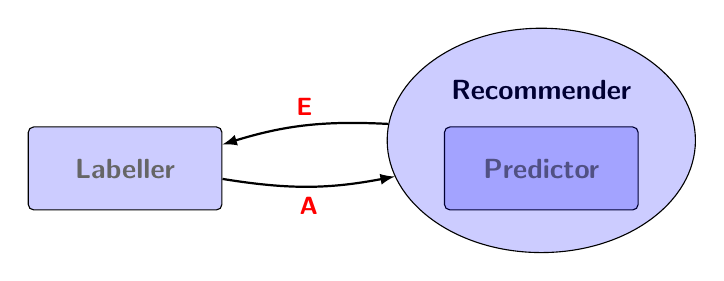
\begin{tikzpicture}[>=latex]

    %
    % Styles for states, and state edges
    %
    \tikzstyle{objectName} = [align=center, font={\sffamily\bfseries}, text=black!60]
    \tikzstyle{bbox} = [draw, very thick, rectangle, rounded corners=2pt, thin,
                          minimum height=3em, minimum width=7em, node distance=8em]
    \tikzstyle{object} = [bbox, objectName, fill=blue!20]
    \tikzstyle{edgePortion} = [black,thick,bend right=10];
    \tikzstyle{dataFlow} = [edgePortion,->];
    \tikzstyle{dataLabel} = [pos=0.5, text centered, text=red, font={\sffamily\bfseries\small}];

    %
    % Position States
    %
    \node[object, name=labeller] {Labeller};
    \node[object, name=predictor, right = of labeller ] {Predictor};
    \node[objectName, name=recommender, above of=predictor, color=black] {Recommender};
    \node[bbox, name=wrapper, ellipse, fill=blue!=20, fill opacity=0.2, fit={(recommender) (predictor)}] {};

    %
    % Connect States via edges
    %
    \draw (labeller)
      edge[dataFlow] node[dataLabel, below]{A}
      (wrapper);
    \draw (wrapper)
      edge[dataFlow] node[dataLabel, above]{E}
      (labeller);
  \end{tikzpicture}
\caption{$\Omega$ design}
\label{fig:omega-design}
\end{figure}

\newpage
\subsection{{\bf Y} design}

All parties contribute to a central database (Figure~\ref{fig:y-design}).

\begin{figure}[ht]
  \centering
  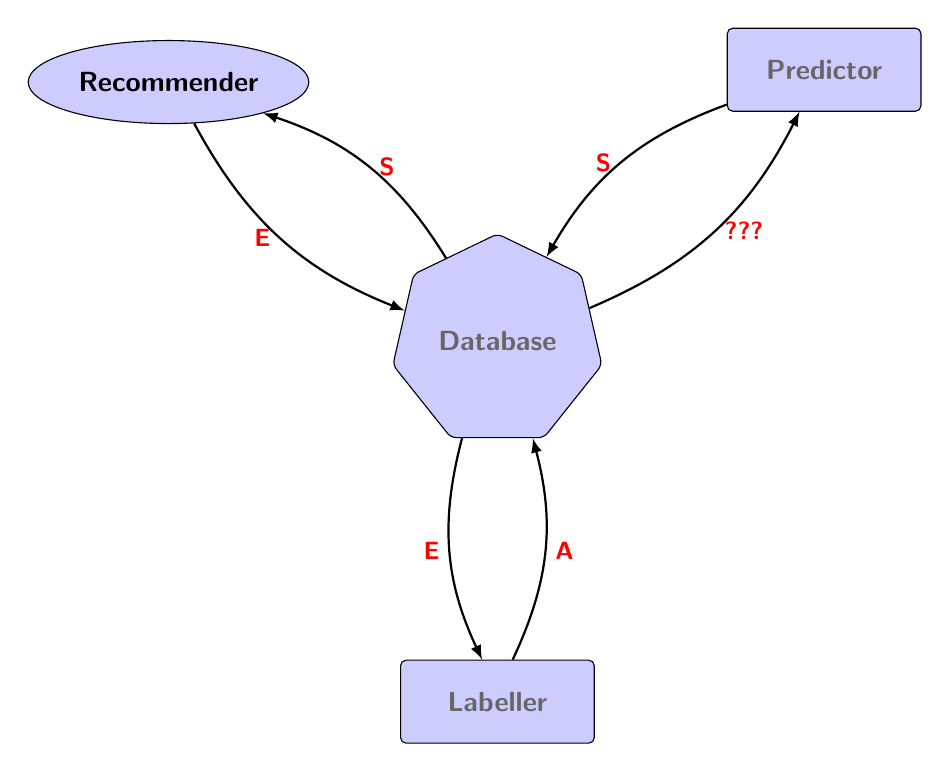
\begin{tikzpicture}[>=latex]

    %
    % Styles for states, and state edges
    %
    \tikzstyle{object} = [draw, very thick, rectangle, rounded corners=2pt, thin, align=center,
                          fill=blue!20, minimum height=3em, minimum width=7em, node distance=8em,
                          font={\sffamily\bfseries}, text=black!60]
    \tikzstyle{edgePortion} = [black,thick,bend right=20];
    \tikzstyle{dataFlow} = [edgePortion,->];
    \tikzstyle{dataLabel} = [pos=0.5, text centered, text=red, font={\sffamily\bfseries\small}];

    %
    % Position States
    %
    \node[object, name=labeller] {Labeller};
    \node[object, name=database, regular polygon, regular polygon sides=7, above = of labeller] {Database};
    \node[object, name=recommender, ellipse, above left = of database, text=black] {Recommender};
    \node[object, name=predictor, above right = of database] {Predictor};

    %
    % Connect States via edges
    %
    \draw (labeller)
      edge[dataFlow] node[dataLabel, right]{A}
      (database);
    \draw (database)
      edge[dataFlow] node[dataLabel, left]{E}
      (labeller);

    \draw (database)
      edge[dataFlow] node[dataLabel, right]{???}
      (predictor);
    \draw (predictor)
      edge[dataFlow] node[dataLabel, left]{S}
      (database);

    \draw (database)
      edge[dataFlow] node[dataLabel, right]{S}
      (recommender);
    \draw (recommender)
      edge[dataFlow] node[dataLabel, left]{E}
      (database);
  \end{tikzpicture}
\caption{{\bf Y} design}
\label{fig:y-design}
\end{figure}

\subsection{Delta design ($\Delta$)}

Each of Labeller, Recommender and Predictor are equal partners (Figure~\ref{fig:delta-design}).

\begin{figure}[ht]
  \centering
  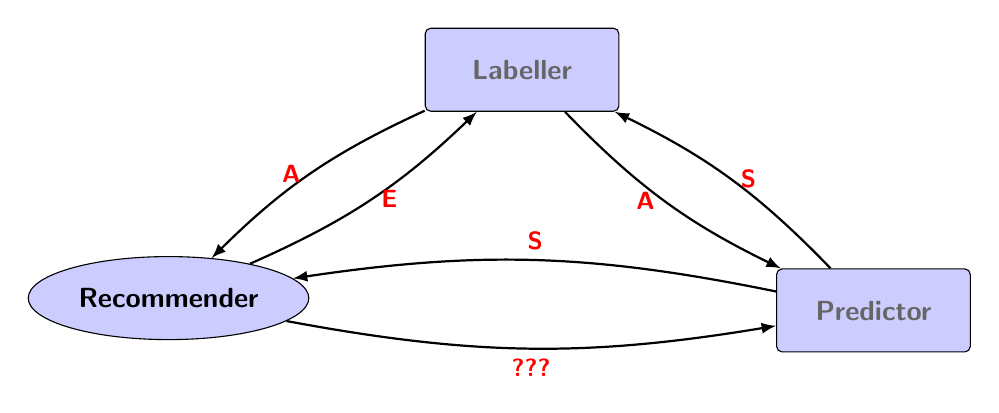
\begin{tikzpicture}[>=latex]

    %
    % Styles for states, and state edges
    %
    \tikzstyle{object} = [draw, very thick, rectangle, rounded corners=2pt, thin, align=center,
                          fill=blue!20, minimum height=3em, minimum width=7em, node distance=8em,
                          font={\sffamily\bfseries}, text=black!60]
    \tikzstyle{edgePortion} = [black,thick,bend right=10];
    \tikzstyle{dataFlow} = [edgePortion,->];
    \tikzstyle{dataLabel} = [pos=0.5, text centered, text=red, font={\sffamily\bfseries\small}];

    %
    % Position States
    %
    \node[object, name=labeller] {Labeller};
    \node[object, name=recommender, ellipse, below left = of labeller, text=black] {Recommender};
    \node[object, name=predictor, below right = of labeller] {Predictor};

    %
    % Connect States via edges
    %
    \draw (labeller)
      edge[dataFlow] node[dataLabel, left]{A}
      (recommender);
    \draw (recommender)
      edge[dataFlow] node[dataLabel, right]{E}
      (labeller);

    \draw (labeller)
      edge[dataFlow] node[dataLabel, left]{A}
      (predictor);
    \draw (predictor)
      edge[dataFlow] node[dataLabel, right]{S}
      (labeller);

    \draw (predictor)
      edge[dataFlow] node[dataLabel, above]{S}
      (recommender);
    \draw (recommender)
      edge[dataFlow] node[dataLabel, below]{???}
      (predictor);
  \end{tikzpicture}
\caption{$\Delta$ design}
\label{fig:delta-design}
\end{figure}



\end{document}
